\tableofcontents
\pagebreak

\section{Свободное движение}
Рассмотрим систему второго порядка в форме В-В:
\begin{equation}
    \ddot{y} + a_1 \dot{y} + a_0 y  = u
\end{equation}
Согласно заданию, выберем три набора корней $(\lambda_1, \lambda_2)$, удовлетворяющих модам из задания (2,3,8)
и найдем небходимы пары коэффициентов $(a_1, a_0)$:
\begin{enumerate}
    \item Нейтральная и устойчивая апериодическая: $\lambda_1 = 0, \lambda_2 = -1$; $a_1 = 1, a_0 = 0$
    \item Нейтральная и неустойчивая апериодическая: $\lambda_1 = 0, \lambda_2 = 0.3$; $a_1 = -0.3, a_0 = 0$
    \item Пара неусточивых колебательных мод: $\lambda_1 = 0.4 + 2i, \lambda_2 = 0.4 - 2i$; $a_1 = -0.8, a_0 = 4.16$
\end{enumerate}


\begin{figure}[h]
    \centering
    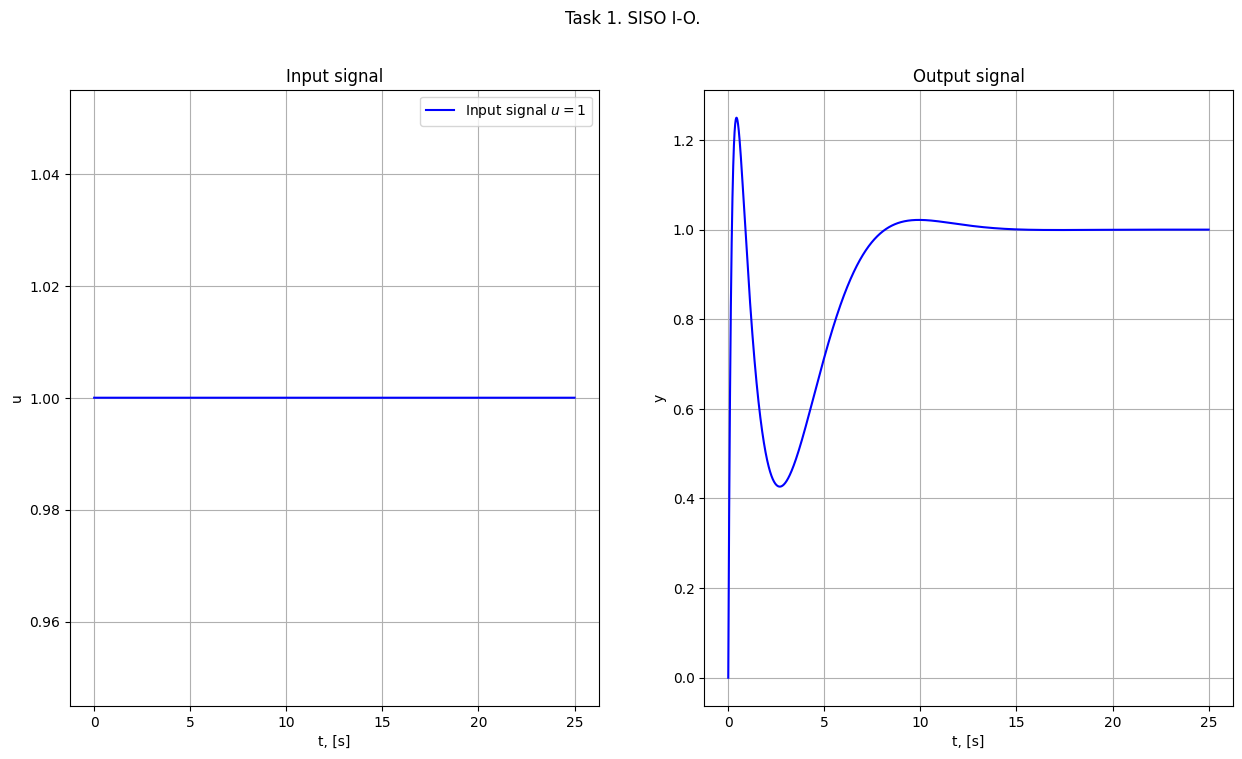
\includegraphics[width=\textwidth]{plot_1_1}
    \caption{\label{fig:The-caption-1}Входные и выходные сигналы систем при нулевых начальных условиях (задание 1)}
\end{figure}

Вычисления пары $(a_1, a_0)$ проведем, воспользовавшись теоремой Виета:
\begin{equation*}
    \begin{cases}
        \lambda_1 + \lambda_2 = - a_1 \\
        \lambda_1 \lambda_2 = a_0
    \end{cases}
\end{equation*}
Согласно корневому критерию, первый набор корней соответствует апериодической системе на границе 
 устойчивости (оба корня действительные, неотрицательны и не кратные), второй - неустойчивой 
 апериодической системе (корни действительные, один из корней имеет положительную действительную часть),
 третий - неустойчивой колебательной системе (пара комплексно сопряженных корней с положительной 
 действительной частью).

 Проведем моделирование поведения систем с нулевыми начальными условиями и при $y(0)=0, \dot y (0) = 1$ 
 (рис. 1 и рис. 2 соответственно).
 

 \begin{figure}[h]
    \centering
    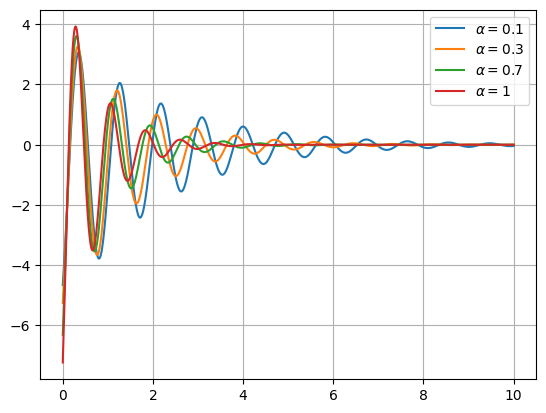
\includegraphics[width=\textwidth]{plot_1_2}
    \caption{\label{fig:The-caption-1}Входные и выходные сигналы систем при ненулевых начальных условиях (задание 1)}
\end{figure}

Заметим, что все системы ведут себя одинаково при задании нулевых начальных условий 
и подаче нулевого управляющего воздействия (они статичны в 0). При задании начальных условий системы
ведут себя согласно аналитически предсказанному корневым критерием.

Аналитическое решение поведения системы (при свободном движении):
\begin{enumerate}
    \item $y(t) = C_1 + C_2 e^{-t}$
    \item $y(t) = C_1 + C_2 e^{0.3t}$
    \item $y(t) = (C_1 \sin{2t} + C_2 \cos{2t}) e^{0.4t}$
\end{enumerate}

\pagebreak

\section{Область устойчивости}
Рассмотрим систему, заданную следующей блок-схемой:
\begin{figure}[h]
    \centering
    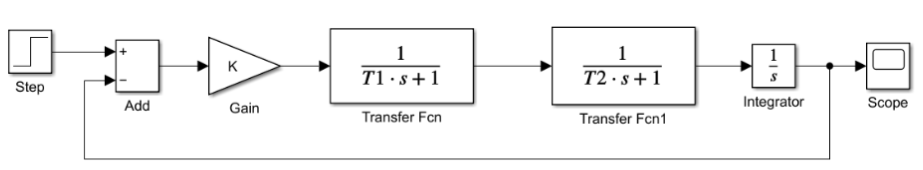
\includegraphics[width=\textwidth]{pic_2_0}
\end{figure}

Можем представить систему передаточной функцией:
\begin{equation*}
    W_0(s) = K, W_1(s) = \frac{1}{T_1 s + 1}, W_2(s) = \frac{1}{T_2 s + 1}, W_3(s)=\frac{1}{s} 
\end{equation*}
\begin{equation*}
    y = W_0W_1W_2W_3(s)[u - y] \implies y = \frac{W_0W_1W_2W_3}{1 + W_0W_1W_2W_3}(s)[u], y = W(s)[u]
\end{equation*}
\begin{equation}
    W(s)=\frac{\frac{K}{s(T_1 s + 1)(T_2 s + 1)}}{1 + \frac{K}{s(T_1 s + 1)(T_2 s + 1)}}=
    \frac{K}{s(T_1 s + 1)(T_2 s + 1) + K}=\frac{K}{T_1 T_2 s^3 + (T_1 + T_2) s^2 + s + K}
\end{equation}
Первый набор корней из первого задания: $\lambda_1 = 0, \lambda_2 = 1$. Таким образом, мы 
не можем выбрать $T_1$. Система с передаточной функцией $\frac{\frac{K}{T_2}}{s^3 + \frac{1}{T_2}s^2 + \frac{K}{T_2}}$
не может быть асимптотически устойчивой согласно критерию Гурвица т.к. условие $a_1 = 0 > 0$ не может быть выполнено.
Граница устойчивости достигается при любом $T_2 \ge 0$ и $K=0$.
Для анализа системы на устойчивость возьмем $\lambda_1 = 1, \lambda_2 = -1$, тогда $T_1=-1, T_2=1$.

Зафиксируем $T_2 = 1$. Запишем критерий Гурвица:
\begin{equation*}
    W(s) = \frac{\frac{K}{T_1}}{s^3 + \frac{T_1 + 1}{T_1} s^2 + \frac{1}{T_1}s + \frac{K}{T_1}}
    \implies 
    \begin{cases}
        \frac{T_1 + 1}{T_1} > 0 \\
        \frac{1}{T_1} > 0 \\
        \frac{K}{T_1} > 0 \\
        \frac{T_1 + 1}{T_1 ^ 2} > \frac{K}{T_1}
    \end{cases} \implies
    \begin{cases}
        T_1 > 0 \\
        K > 0 \\
        K < 1 + \frac{1}{T_1}
    \end{cases}
\end{equation*}
Таким образом, зона устойчивости ограничена прямыми $K=0$, $T_1=0$ и гиперболой $K = 1 + \frac{1}{T_1}$ (рис. 3).

Зафиксируем $T_1 = -1$. Запишем критерий Гурвица:
\begin{equation*}
    W(s) = \frac{\frac{K}{T_2}}{s^3 + \frac{1 - T_2}{T_2} s^2 - \frac{1}{T_2}s - \frac{K}{T_2}}
    \implies 
    \begin{cases}
        \frac{1 - T_2}{T_2} > 0 \\
        -\frac{1}{T_2} > 0 \\
        -\frac{K}{T_2} > 0 \\
        \frac{T_2 - 1}{T_2 ^ 2} > -\frac{K}{T_2}
    \end{cases} \implies
    \begin{cases}
        T_2 < 0 \\
        K > 0 \\
        K < -1 + \frac{1}{T_2}
        % -\frac{T_2 - 1}{T_2 } > K 
    \end{cases} \implies \varnothing
\end{equation*}
Таким образом, система не имеет зоны устойчивости.

Выполним моделирование систем, заданных следующими тройками параметров $K, T_1, T_2$ (рис. 4): (1,1,1) - устойчиваяя
, (2,1,1) - на границе устойчивости и (3,2,1) - неустойчивая.

\begin{figure}[]
    \centering
    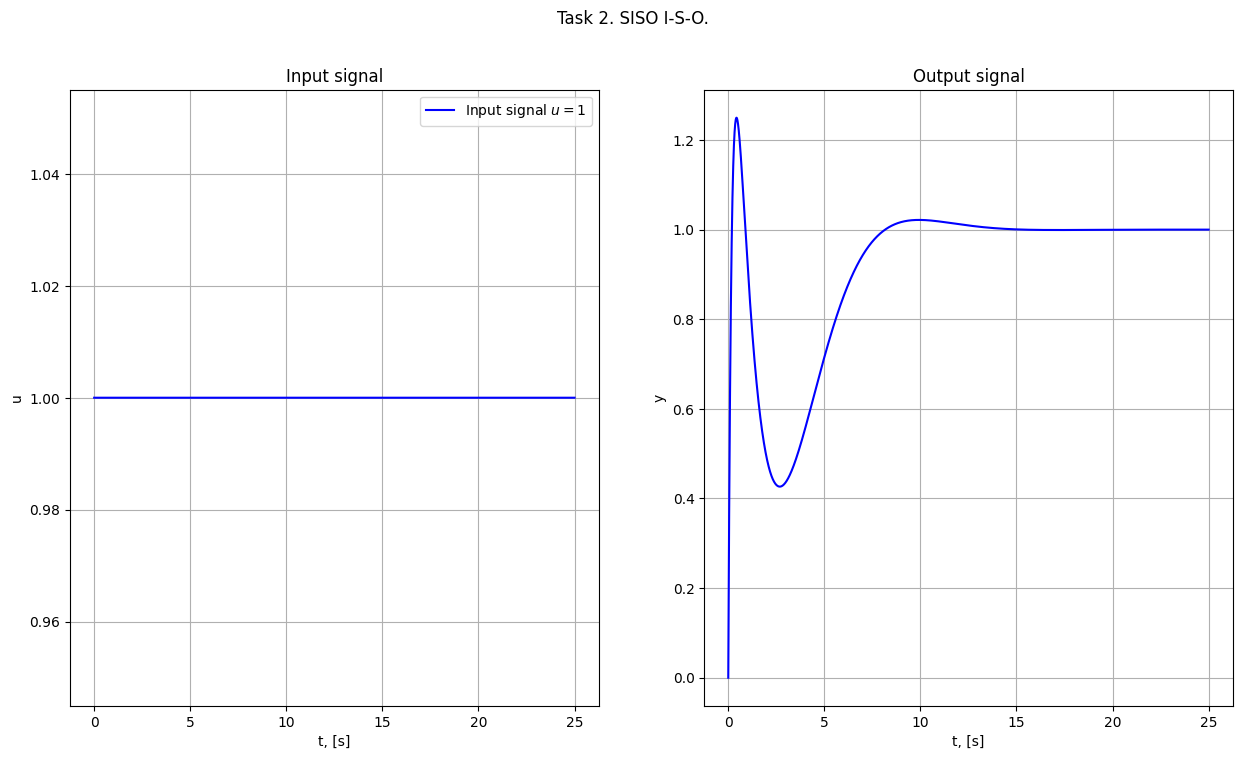
\includegraphics[width=300px, height=260px]{plot_2_1}
    \caption{\label{fig:The-caption-1}Зона устойчивости при фиксированном $T_2=1$ (задание 2)}
\end{figure}
\begin{figure}[]
    \centering
    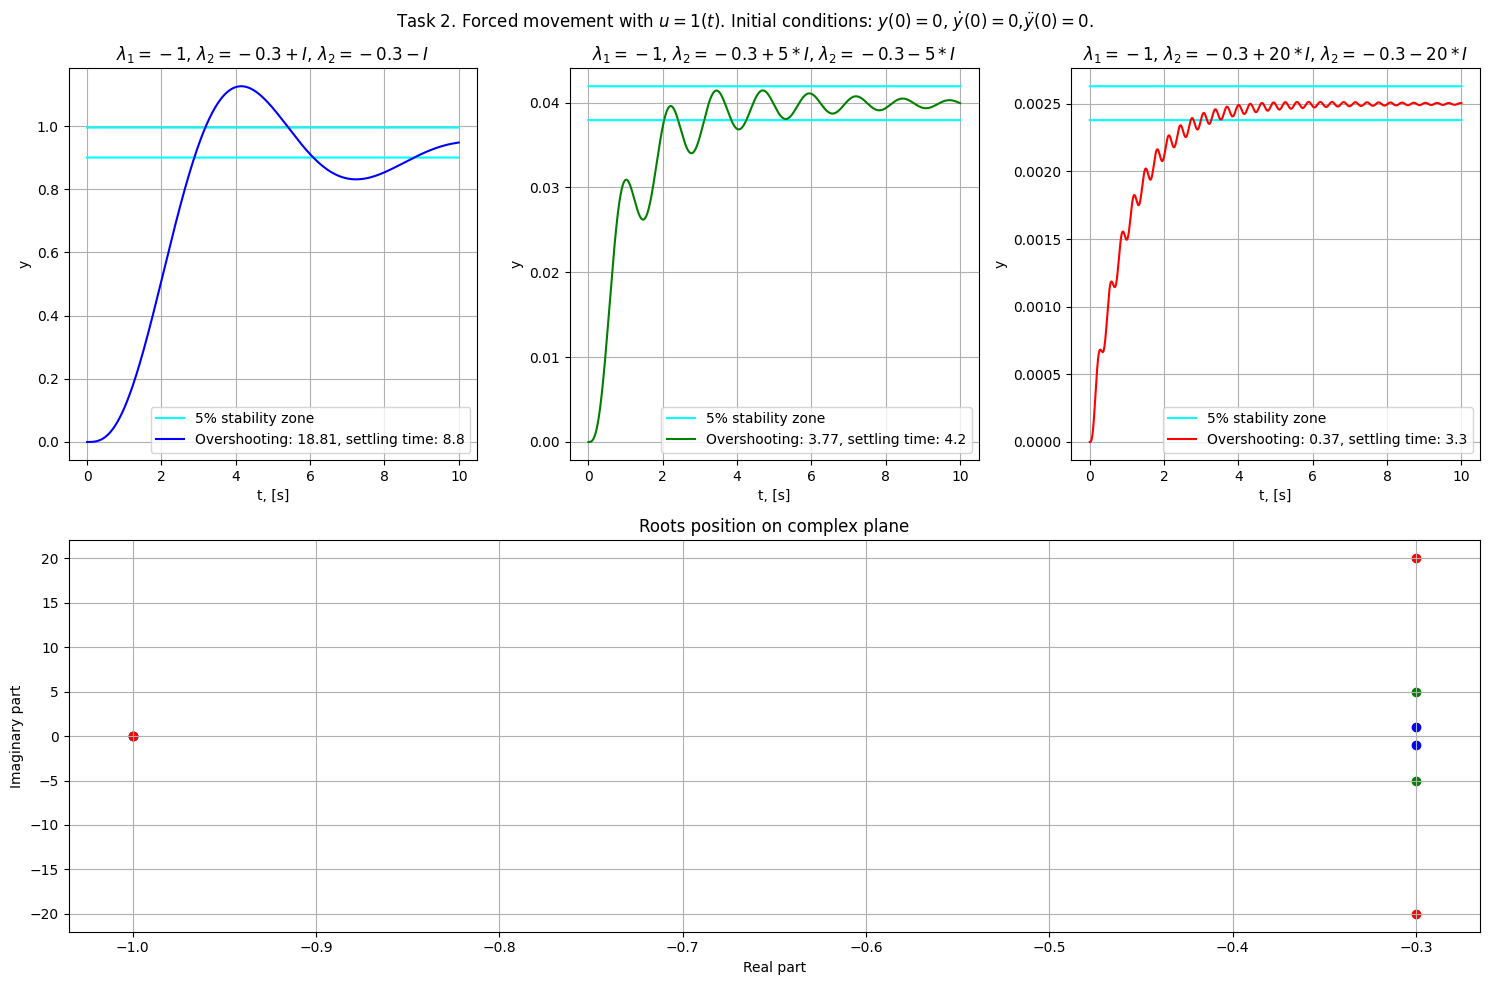
\includegraphics[width=\textwidth]{plot_2_2}
    \caption{\label{fig:The-caption-1}Моделирование систем с разными типами устойчивости (задание 2)}
\end{figure}
\pagebreak

\section{Автономный генератор}
Рассмотрим систему вида:
\begin{equation}
    \begin{cases}
        \dot x = A x \\
        y = C x
    \end{cases}
\end{equation}
Согласно теории однородных дифференциальных уравнений, можем записать решение системы следующим образом:
\begin{equation}
    x(t) = e^{At}x(0) \implies y(t) = C e^{At}x(0)
\end{equation}
Желаемый вид выходного сигнала согласно условию: $y(t) = -\sin{5t} + e^{-7}\sin{9t}$. Решение такого вида
достигается при следующем наборе корней характеристического полинома матрицы $A$:\\ $\lambda_1 = 5i, \lambda_2 = -5i
,\lambda_3 = -7 + 9i,\lambda_4 = -7 - 9i$.

Представим матрицу $A$ в Жордановой нормальной форме (изменим базис состояний). Тогда, можем записать систему $(3)$ в виде:
\begin{equation}
    A = TJT^{-1},
    \begin{cases}
        \dot x = TJT^{-1}x \\
        y = C x
    \end{cases}
    \implies 
    \begin{cases}
        x(t) = Te^{Jt}T^{-1}x(0) = Te^{Jt}\widetilde{x}(0) \\
        y(t) = C Te^{Jt}T^{-1}x(0) = \widetilde{C}e^{Jt}\widetilde{x}(0)
    \end{cases},
    \widetilde{x} = T^{-1}x, \widetilde{C} = CT
\end{equation}
\begin{equation*}
    J = \begin{bmatrix}
        0 & 5 & 0 & 0   \\
        -5 & 0 & 0 & 0  \\
        0 & 0 & -7 & 9 \\
        0 & 0 & -9 & -7
        \end{bmatrix},
    e^{Jt} = \begin{bmatrix}
        \cos{5t} & \sin{5t} & 0 & 0   \\
        -\sin{5t} & \cos{5t} & 0 & 0  \\
        0 & 0 & e^{-7}\cos{9t} & e^{-7}\sin{9t} \\
        0 & 0 & -e^{-7}\sin{9t} & e^{-7}\cos{9t}
        \end{bmatrix}
\end{equation*}
\begin{figure}[h]
    \centering
    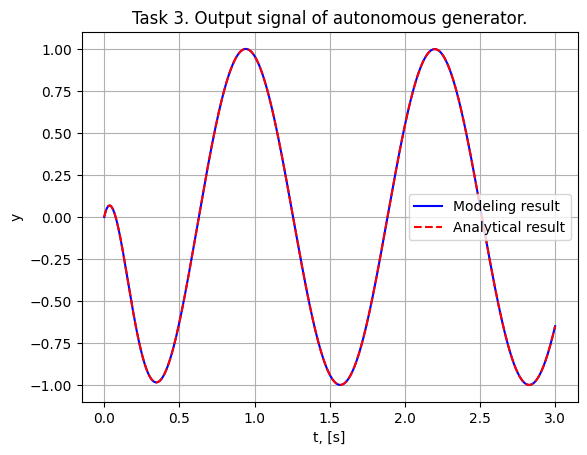
\includegraphics[width=300px, height=260px]{plot_3_1}
    \caption{\label{fig:The-caption-1}Выход автономного генератора (задание 3)}
\end{figure}

Найдем подходящие матрицы $\widetilde{C}$ и $\widetilde{x}(0)$ для получения требуемого выходного сигнала:
\begin{gather*}
    y(t) = \widetilde{C}e^{Jt}\widetilde{x}(0) =
    \begin{bmatrix}
        \tilde{c}_1 & \tilde{c}_2 & \tilde{c}_3 & \tilde{c}_4 
    \end{bmatrix} 
    \begin{bmatrix}
        \cos{5t} & \sin{5t} & 0 & 0   \\
        -\sin{5t} & \cos{5t} & 0 & 0  \\
        0 & 0 & e^{-7}\cos{9t} & e^{-7}\sin{9t} \\
        0 & 0 & -e^{-7}\sin{9t} & e^{-7}\cos{9t}
        \end{bmatrix}
    \begin{bmatrix}
        \tilde{x}(0)_1\\
        \tilde{x}(0)_2\\
        \tilde{x}(0)_3\\
        \tilde{x}(0)_4
    \end{bmatrix}
     = \\ (\tilde{c}_1\tilde{x}(0)_1 + \tilde{c}_2\tilde{x}(0)_2) \cos{5t} +
    (\tilde{c}_1\tilde{x}(0)_2 - \tilde{c}_2\tilde{x}(0)_1) \sin{5t} + 
    (\tilde{c}_3\tilde{x}(0)_3 + \tilde{c}_4\tilde{x}(0)_4) e^{-7t}\cos{9t} + \\
    (\tilde{c}_3\tilde{x}(0)_4 - \tilde{c}_4\tilde{x}(0)_3) e^{-7t}\sin{9t} = 
    y(t) = -\sin{5t} + e^{-7}\sin{9t} \implies \\
    \implies
    \begin{cases}
        (\tilde{c}_1\tilde{x}(0)_1 + \tilde{c}_2\tilde{x}(0)_2) = 0 \\
        (\tilde{c}_1\tilde{x}(0)_2 - \tilde{c}_2\tilde{x}(0)_1) = -1 \\
        (\tilde{c}_3\tilde{x}(0)_3 + \tilde{c}_4\tilde{x}(0)_4) = 0 \\
        (\tilde{c}_3\tilde{x}(0)_4 - \tilde{c}_4\tilde{x}(0)_3) = 1
    \end{cases},
    \begin{cases}
        \tilde{c}_2 = \tilde{x}(0)_1 = 0 \\
        \tilde{c}_4 = \tilde{x}(0)_3 = 0 \\
        \tilde{c}_3 = \tilde{x}(0)_2 = \tilde{x}(0)_4 = 1 \\
        \tilde{c}_1 = -1
    \end{cases}
\end{gather*}
Таким образом:
\begin{equation*}
    \widetilde{C} = \begin{bmatrix}
        -1 & 0 & 1 & 0
    \end{bmatrix},
    \widetilde{x}(0) = \begin{bmatrix}
        0 & 1 & 0 & 1
    \end{bmatrix}^T
\end{equation*}
Проведем моделирование системы $(5)$, зная матрицы $\widetilde{x}(0)$ и $\widetilde{C}$ (рис. 5). Как видно, 
выход системы, заданной найденными матрицами идентичен желаемому выходу.

\pagebreak

\section{Изучение канонической управляемой формы: фазовые портреты}
Рассмотрим систему второго порядка $(1)$ в свободном движении. Возьмем последний набор корней из 1-го задания:
$\lambda_1 = 0.4 + 2 i$, $\lambda_1 = 0.4 - 2 i$. Данная система неустойчива и при ненулевых начальных условиях
расходится. Проведем моделирование в форме В-В и в канонической управляемой форме (рис. 6).
\begin{figure}[h]
    \centering
    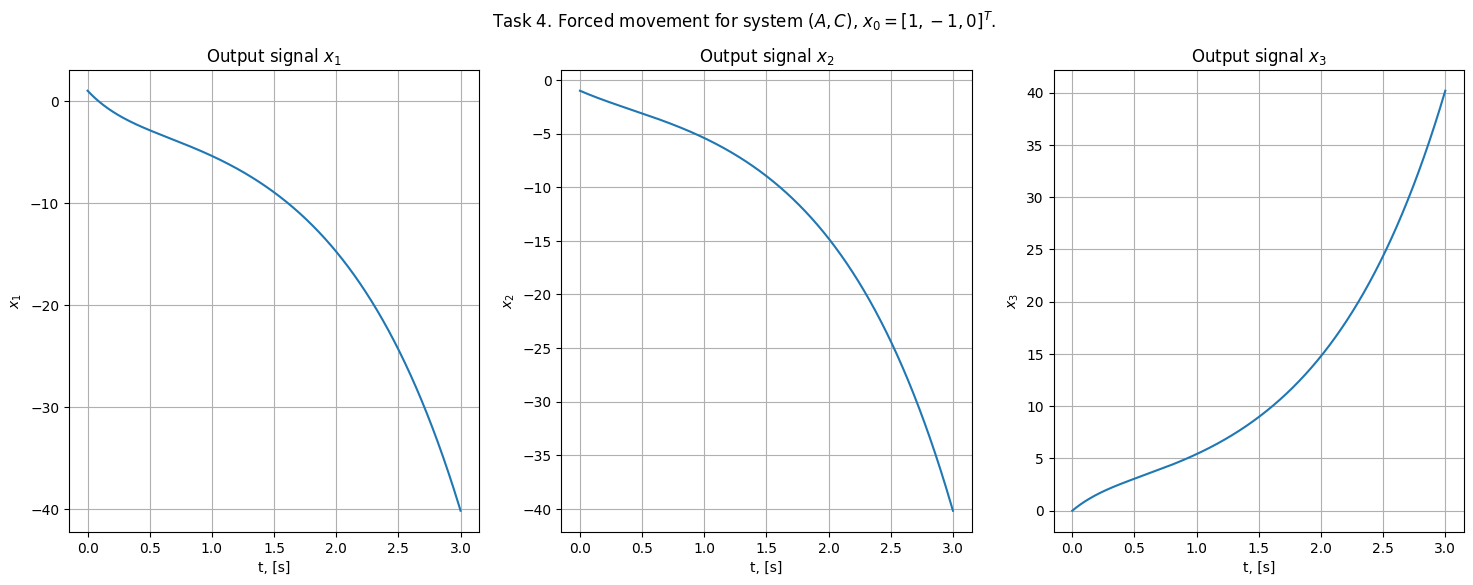
\includegraphics[width=\textwidth]{plot_4_1}
    \caption{\label{fig:The-caption-1}Сравнение фазовых портретов в форме В-В и в канонической
    управляемой форме (задание 4)}
\end{figure}

Можем заметить, что фазовые портреты идентичны. 
\pagebreak

\section{Выводы}

\pagebreak